\chapter{Project Requirements}
\label{ch:requirements}

This chapter describes the functional and non-functional requirements of the Urdu-Native Voice Agent project, including key use cases and the domain model.

\section{Use Cases}

Given the interactive nature of the Urdu-Native Voice Agent as an end-user application with multiple stakeholder interactions, use cases are the most suitable technique for capturing functional requirements.

\subsection{Use Case: Inbound Property Inquiry Call}

\begin{table}[!htbp]
\centering
\caption{Use Case Attributes --- Inbound Property Inquiry Call}
\label{tab:uc-inbound-attributes}
\renewcommand{\arraystretch}{1.2}
\begin{tabular}{|l|p{9cm}|}
\hline
\textbf{Attribute} & \textbf{Description} \\ \hline
Scope & Urdu-Native Voice Agent --- Inbound Call Processing \\ \hline
Level & User-Goal \\ \hline
Primary Actor & Potential Customer \\ \hline
Preconditions & Telephony gateway operational, ASR/TTS models loaded, Property database indexed \\ \hline
Postconditions & Customer query resolved or escalated, Call logged and summarized \\ \hline
\end{tabular}
\end{table}

\begin{figure}[!htbp]
\centering
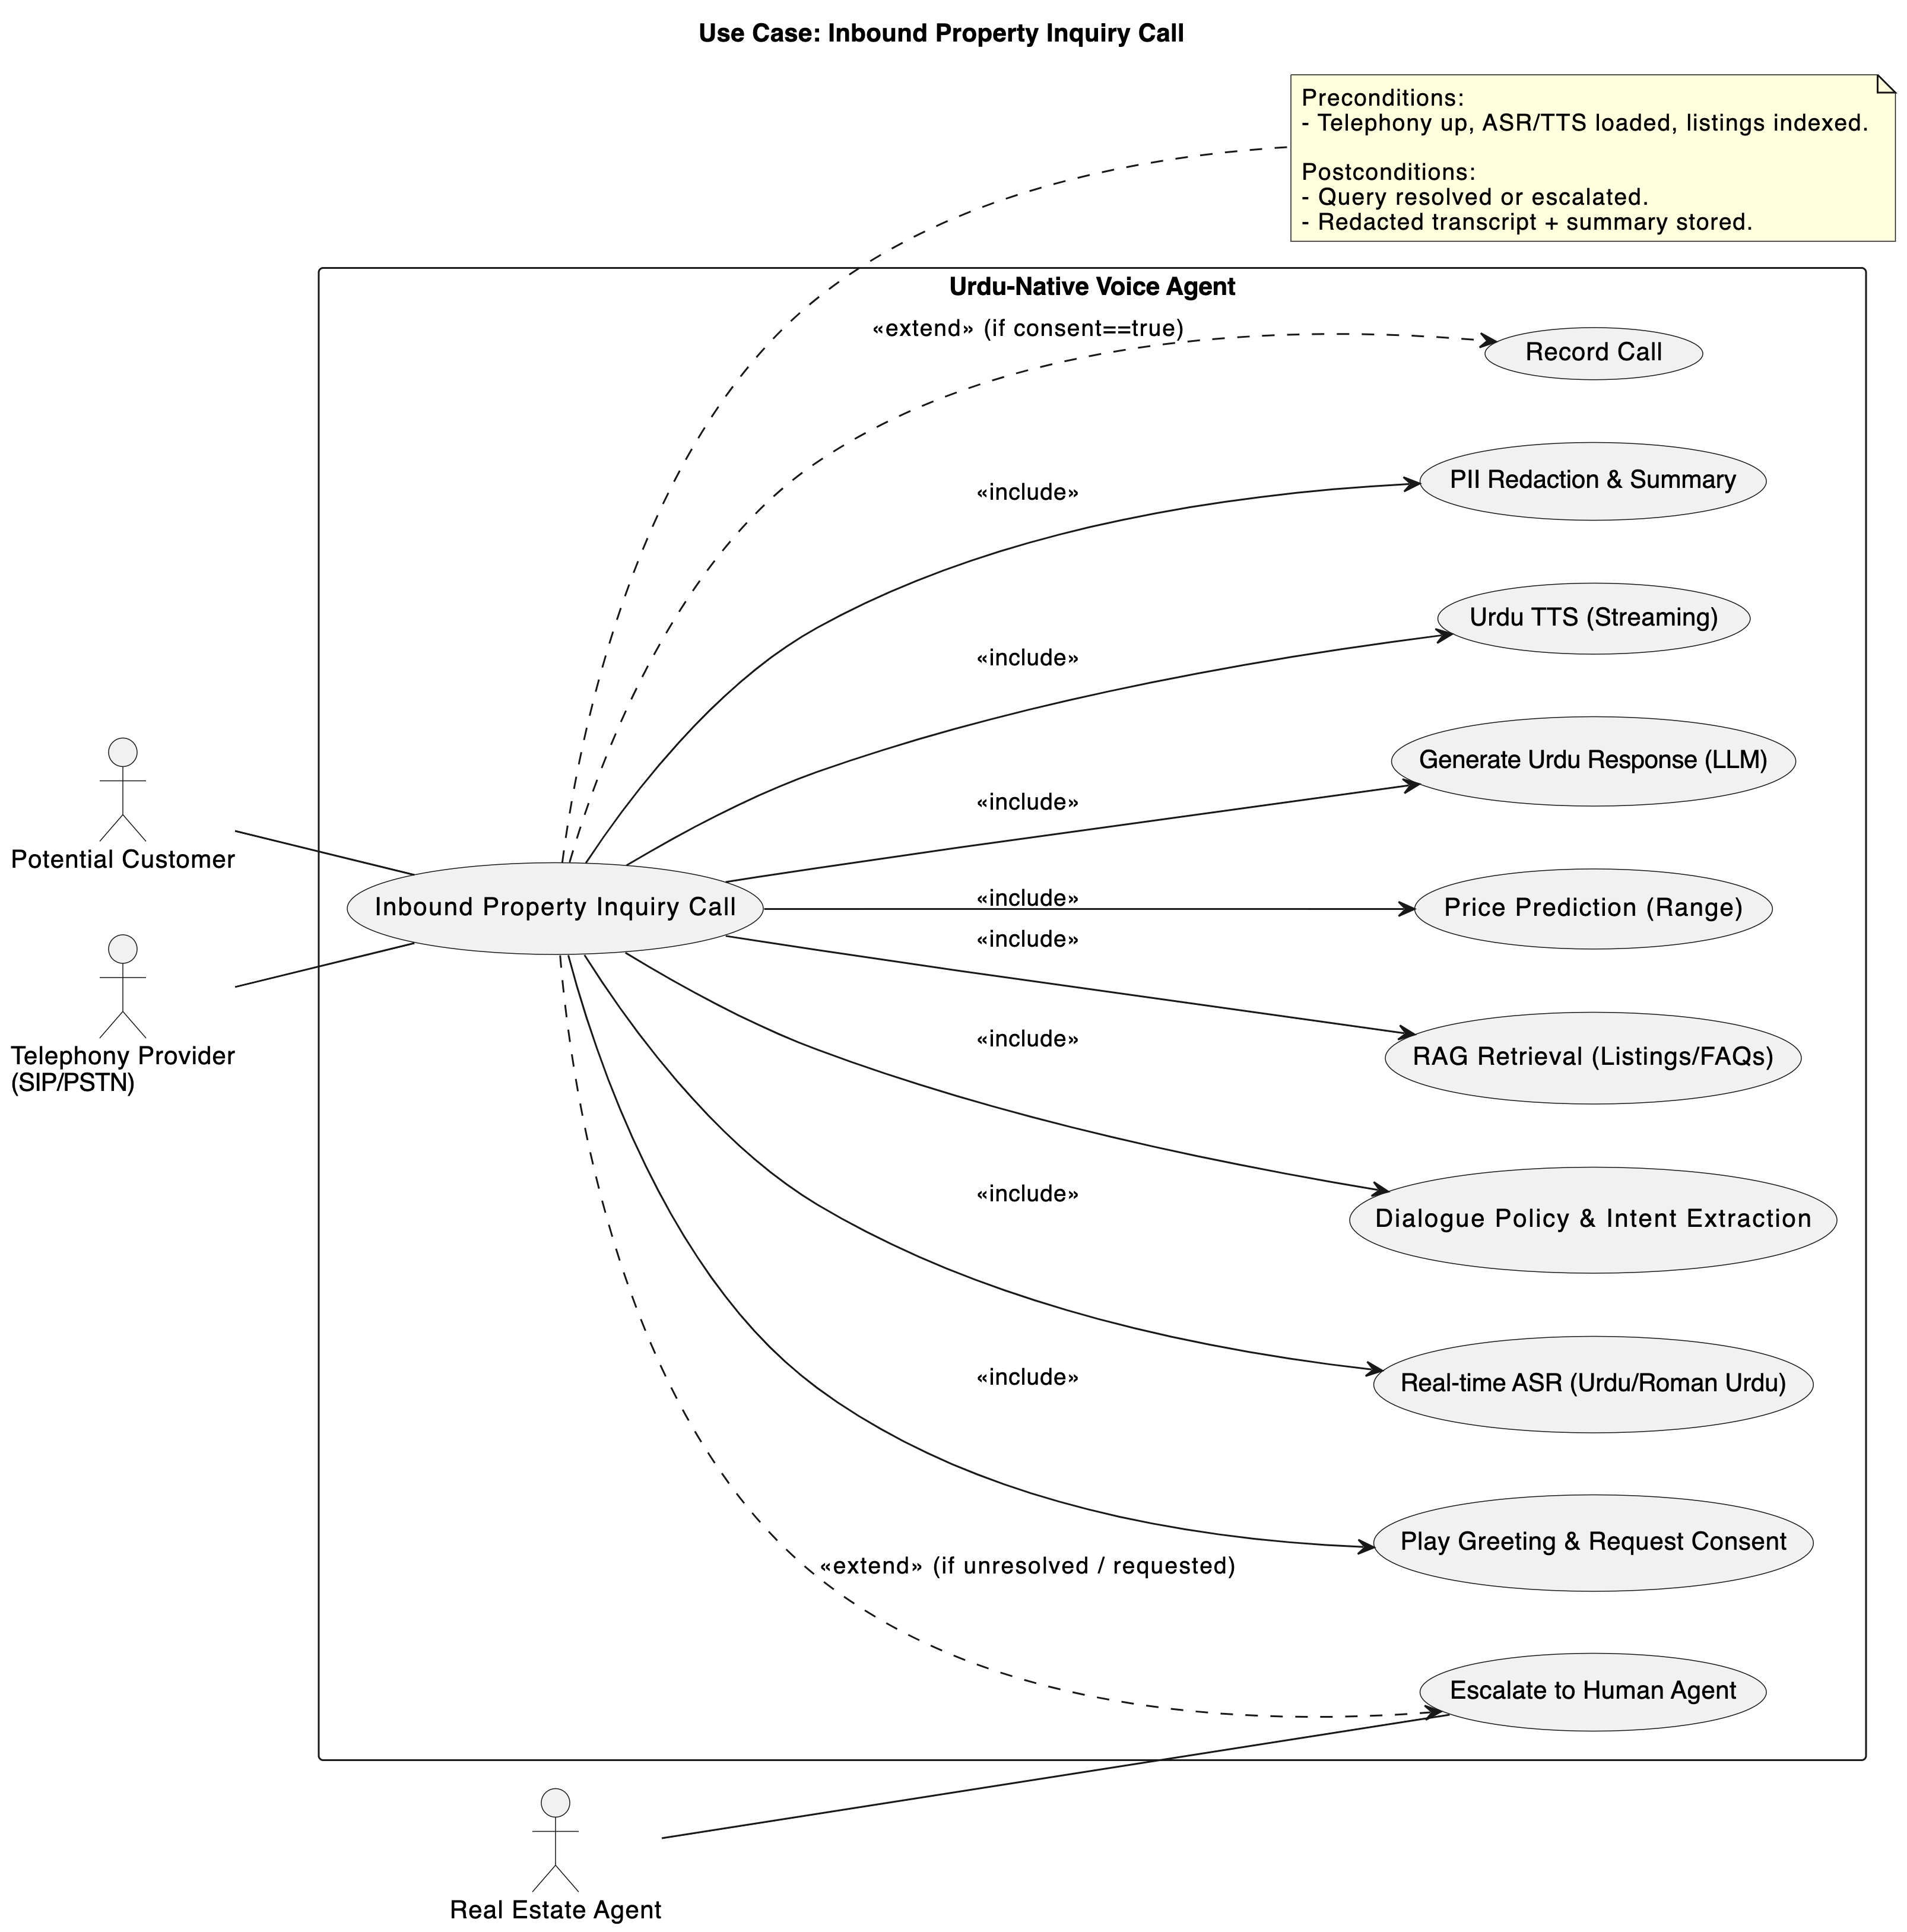
\includegraphics[width=0.95\textwidth]{ThesisFigs/Use Case Diagram_FYP.drawio}
\caption{Use Case Diagram --- Inbound Property Inquiry Call}
\label{fig:uc-inbound}
\end{figure}

\textbf{Main Success Scenario:}
\begin{enumerate}
    \item Customer calls the advertised number
    \item System answers, plays greeting, and requests consent for recording
    \item Customer speaks inquiry in Urdu (e.g., ``Lahore mein 10 marla plot ki price kya hai?'')
    \item ASR transcribes speech to text in real-time
    \item Dialogue Manager extracts intent and key entities (location, type, size)
    \item RAG agent retrieves relevant listings; price-prediction provides estimate
    \item LLM formulates a natural Urdu response
    \item TTS converts response to speech and plays to user
    \item Conversation continues until query is resolved
    \item System logs redacted transcript and generates summary
\end{enumerate}

\subsection{Use Case: Outbound Lead Qualification Call}

\begin{table}[!htbp]
\centering
\caption{Use Case Attributes --- Outbound Lead Qualification Call}
\label{tab:uc-outbound-attributes}
\renewcommand{\arraystretch}{1.2}
\begin{tabular}{|l|p{9cm}|}
\hline
\textbf{Attribute} & \textbf{Description} \\ \hline
Scope & Urdu-Native Voice Agent --- Outbound Campaign \\ \hline
Level & User-Goal \\ \hline
Primary Actor & System Agent \\ \hline
Preconditions & Lead list loaded, Telephony operational, Calling hours appropriate \\ \hline
Postconditions & Lead qualified/disqualified, Call result logged, Follow-up scheduled \\ \hline
\end{tabular}
\end{table}

\begin{figure}[!htbp]
\centering
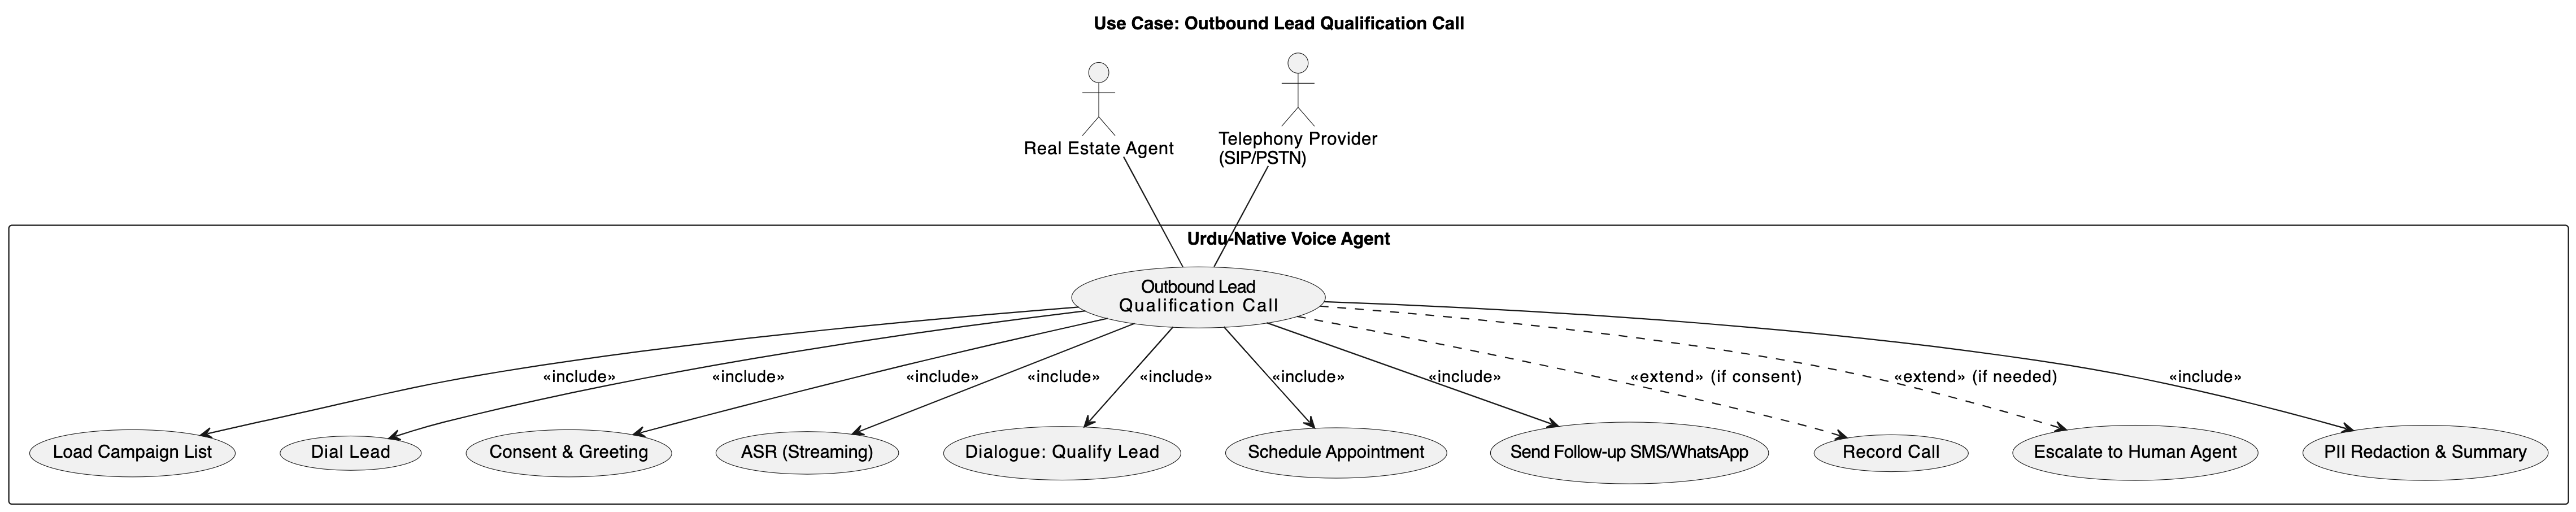
\includegraphics[width=0.95\textwidth]{ThesisFigs/Outbound Use case.drawio}
\caption{Use Case Diagram --- Outbound Lead Qualification Call}
\label{fig:uc-outbound}
\end{figure}

\textbf{Main Success Scenario:}
\begin{enumerate}
    \item System initiates outbound call to lead
    \item System identifies itself as AI agent and requests consent
    \item Customer engages in conversation
    \item ASR transcribes customer responses
    \item Dialogue Manager qualifies lead based on budget, timeline, and preferences
    \item System provides relevant property suggestions
    \item System attempts to schedule follow-up or viewing
    \item Conversation results logged in CRM; lead status updated
\end{enumerate}

\subsection{Use Case: Property Price Estimation Request}

\begin{table}[!htbp]
\centering
\caption{Use Case Attributes --- Property Price Estimation Request}
\label{tab:uc-price-attributes}
\renewcommand{\arraystretch}{1.2}
\begin{tabular}{|l|p{9cm}|}
\hline
\textbf{Attribute} & \textbf{Description} \\ \hline
Scope & Urdu-Native Voice Agent --- Price Estimation \\ \hline
Level & User-Goal \\ \hline
Primary Actor & Customer \\ \hline
Preconditions & Property database contains comparable listings, Price prediction model operational \\ \hline
Postconditions & Price estimate provided with confidence level, Comparable properties cited \\ \hline
\end{tabular}
\end{table}

\begin{figure}[!htbp]
\centering
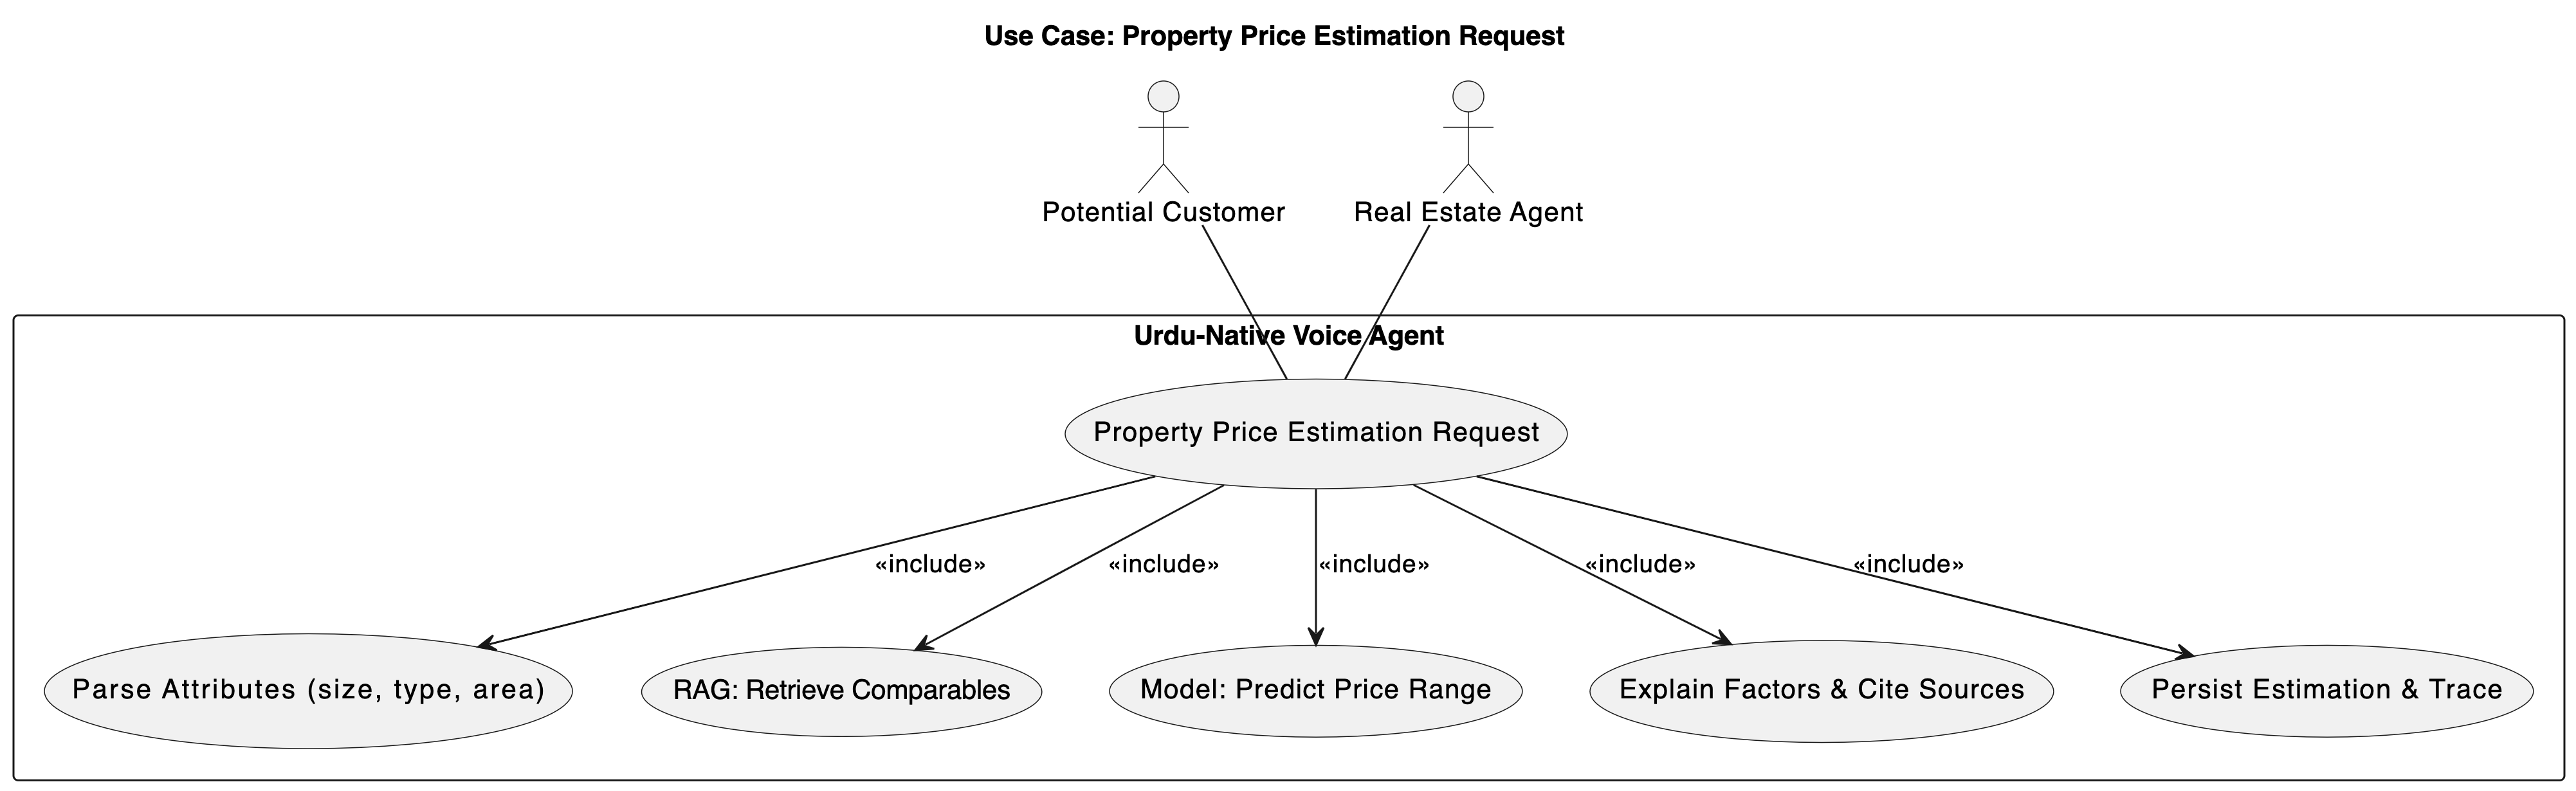
\includegraphics[width=0.95\textwidth]{ThesisFigs/PricePrediction}
\caption{Use Case Diagram --- Property Price Estimation Request}
\label{fig:uc-price}
\end{figure}

\textbf{Main Success Scenario:}
\begin{enumerate}
    \item Customer describes property features
    \item ASR transcribes property description
    \item Dialogue Manager extracts property attributes
    \item RAG engine finds comparable properties
    \item Price prediction model calculates estimate range
    \item System provides estimate with confidence level
    \item System cites comparable properties used for estimation
    \item Customer may ask follow-up questions for additional context
\end{enumerate}

\subsection{Use Case: Post-Call Analytics and Review}

\begin{figure}[!htbp]
\centering
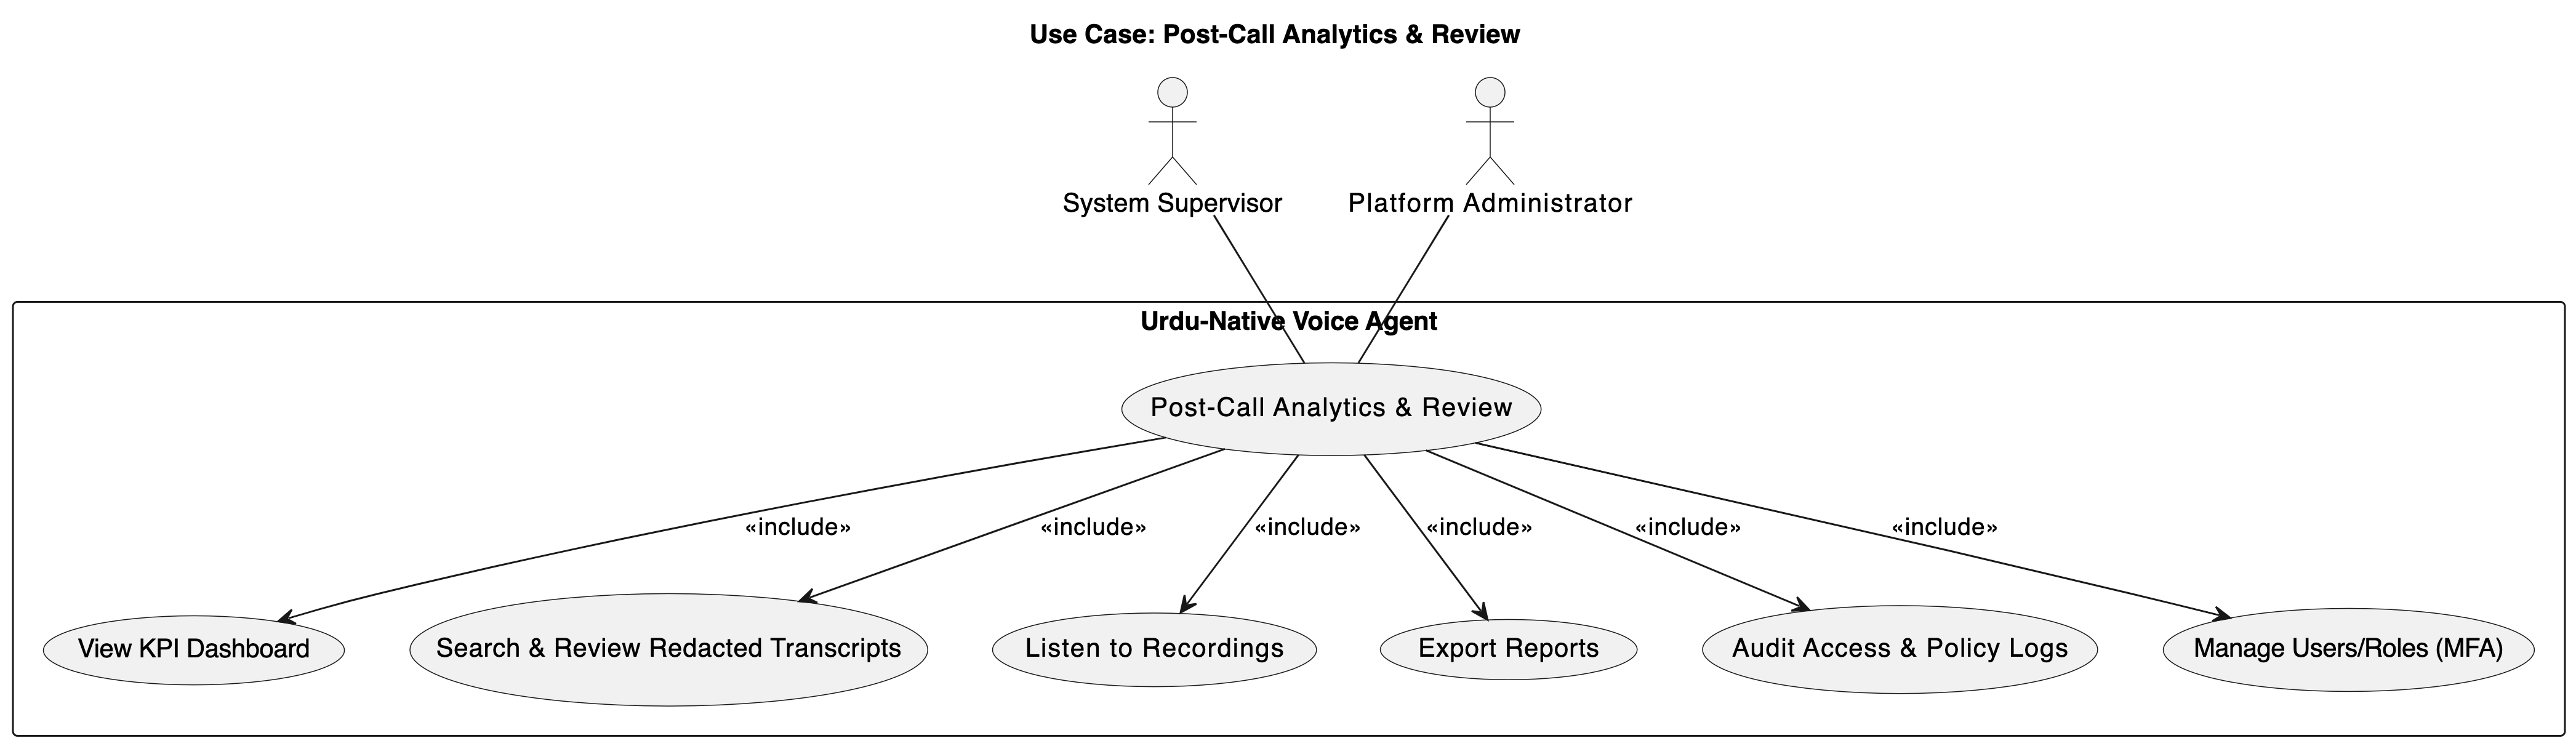
\includegraphics[width=0.95\textwidth]{ThesisFigs/PostCallAnalytics.drawio}
\caption{Use Case Diagram --- Post-Call Analytics and Review}
\label{fig:uc-analytics}
\end{figure}

\textbf{Main Success Scenario:}
\begin{enumerate}
    \item Supervisor logs into analytics dashboard
    \item System authenticates user and loads dashboard interface
    \item Supervisor selects date range and applies filters
    \item System retrieves and displays filtered call data
    \item Supervisor reviews conversation flow and key metrics
    \item System highlights key moments and sentiment analysis
    \item Supervisor exports performance reports as PDF/CSV
\end{enumerate}

%----------------------------------------------------------------------
\section{Functional Requirements}

This section describes the functional requirements organized by module.

\subsection{Module 1: Automatic Speech Recognition (ASR)}
\begin{enumerate}
    \item FR-1.1: The system shall transcribe spoken Urdu from narrowband telephony audio with Word Error Rate (WER) $<$20\%
    \item FR-1.2: The system shall support real-time streaming transcription with partial results
    \item FR-1.3: The system shall normalize and transcribe Roman Urdu input into standardized text
    \item FR-1.4: The system shall implement lexicon biasing for at least 500 domain-specific terms
    \item FR-1.5: The system shall provide per-token confidence scores for transcription assessment
\end{enumerate}

\subsection{Module 2: Dialogue Manager \& LLM Policy}
\begin{enumerate}
    \item FR-2.1: The system shall use a locally hosted LLM to generate contextually appropriate Urdu responses
    \item FR-2.2: The system shall classify user intent with $>$90\% accuracy
    \item FR-2.3: The system shall integrate with RAG module to incorporate retrieved facts into responses
    \item FR-2.4: The system shall enforce safety policies, preventing unverified information sharing
    \item FR-2.5: The system shall maintain conversation context across multiple dialogue turns
\end{enumerate}

\subsection{Module 3: RAG \& Price-Prediction Agent}
\begin{enumerate}
    \item FR-3.1: The system shall retrieve top-3 most relevant property listings from vector database
    \item FR-3.2: The system shall provide price range estimate citing features used for prediction
    \item FR-3.3: The price-prediction model shall achieve MAPE $<$15\% on held-out test set
    \item FR-3.4: The system shall track provenance for all factual statements and estimates
    \item FR-3.5: The system shall update property database with new listings and price changes
\end{enumerate}

\subsection{Module 4: Text-to-Speech (TTS)}
\begin{enumerate}
    \item FR-4.1: The system shall synthesize Urdu speech with Mean Opinion Score (MOS) $>$3.5
    \item FR-4.2: The TTS system shall begin audio playback as soon as partial audio is ready
    \item FR-4.3: The system shall support SSML-style markup for pauses and emphasis
    \item FR-4.4: The system shall handle Urdu text normalization and proper pronunciation
\end{enumerate}

\subsection{Module 5: Telephony \& Voice Gateway}
\begin{enumerate}
    \item FR-5.1: The system shall connect to SIP trunk to place and receive telephone calls
    \item FR-5.2: The system shall play consent message at call start and only record if consent given
    \item FR-5.3: The system shall manage multiple concurrent call sessions
    \item FR-5.4: The system shall handle call transfer and escalation to human agents
\end{enumerate}

\subsection{Module 6: Analytics Dashboard}
\begin{enumerate}
    \item FR-6.1: The system shall automatically redact PII from call transcripts with $>$95\% recall
    \item FR-6.2: The dashboard shall display key metrics: call volume, handling time, conversion rate
    \item FR-6.3: The system shall generate automated call summaries with key conversation points
    \item FR-6.4: The system shall provide role-based access control for different user types
\end{enumerate}

%----------------------------------------------------------------------
\section{Non-Functional Requirements}

\subsection{Performance Requirements}
\begin{enumerate}
    \item PER-1: The system shall process audio streams with latency suitable for real-time conversation
    \item PER-2: The system shall handle multiple concurrent sessions without degradation
    \item PER-3: The system shall complete database queries within acceptable time limits
    \item PER-4: The system shall load and process models efficiently within hardware constraints
\end{enumerate}

\subsection{Reliability Requirements}
\begin{enumerate}
    \item REL-1: The system shall achieve high availability during operational hours
    \item REL-2: The system shall have robust error handling and recovery mechanisms
    \item REL-3: The system shall provide data backup and recovery capabilities
    \item REL-4: The system shall maintain data integrity for all call records
\end{enumerate}

\subsection{Security Requirements}
\begin{enumerate}
    \item SEC-1: The system shall encrypt all data transmission using secure protocols
    \item SEC-2: The system shall store sensitive data using appropriate encryption standards
    \item SEC-3: The system shall implement session management with timeout policies
    \item SEC-4: The system shall require authentication for administrative functions
    \item SEC-5: The system shall maintain audit logs for all user actions and system events
\end{enumerate}

\subsection{Usability Requirements}
\begin{enumerate}
    \item USE-1: The system shall allow supervisors to review transcripts through intuitive interface
    \item USE-2: The system shall provide responsive design supporting various screen sizes
    \item USE-3: The system shall offer clear navigation and organization of features
    \item USE-4: The system shall provide adequate feedback for user actions and system status
\end{enumerate}

%----------------------------------------------------------------------
\section{Domain Model}

Figure~\ref{fig:domain-model} presents the domain model for the Urdu-Native Voice Agent, showing core entities and their relationships.

\begin{figure}[!htbp]
\centering
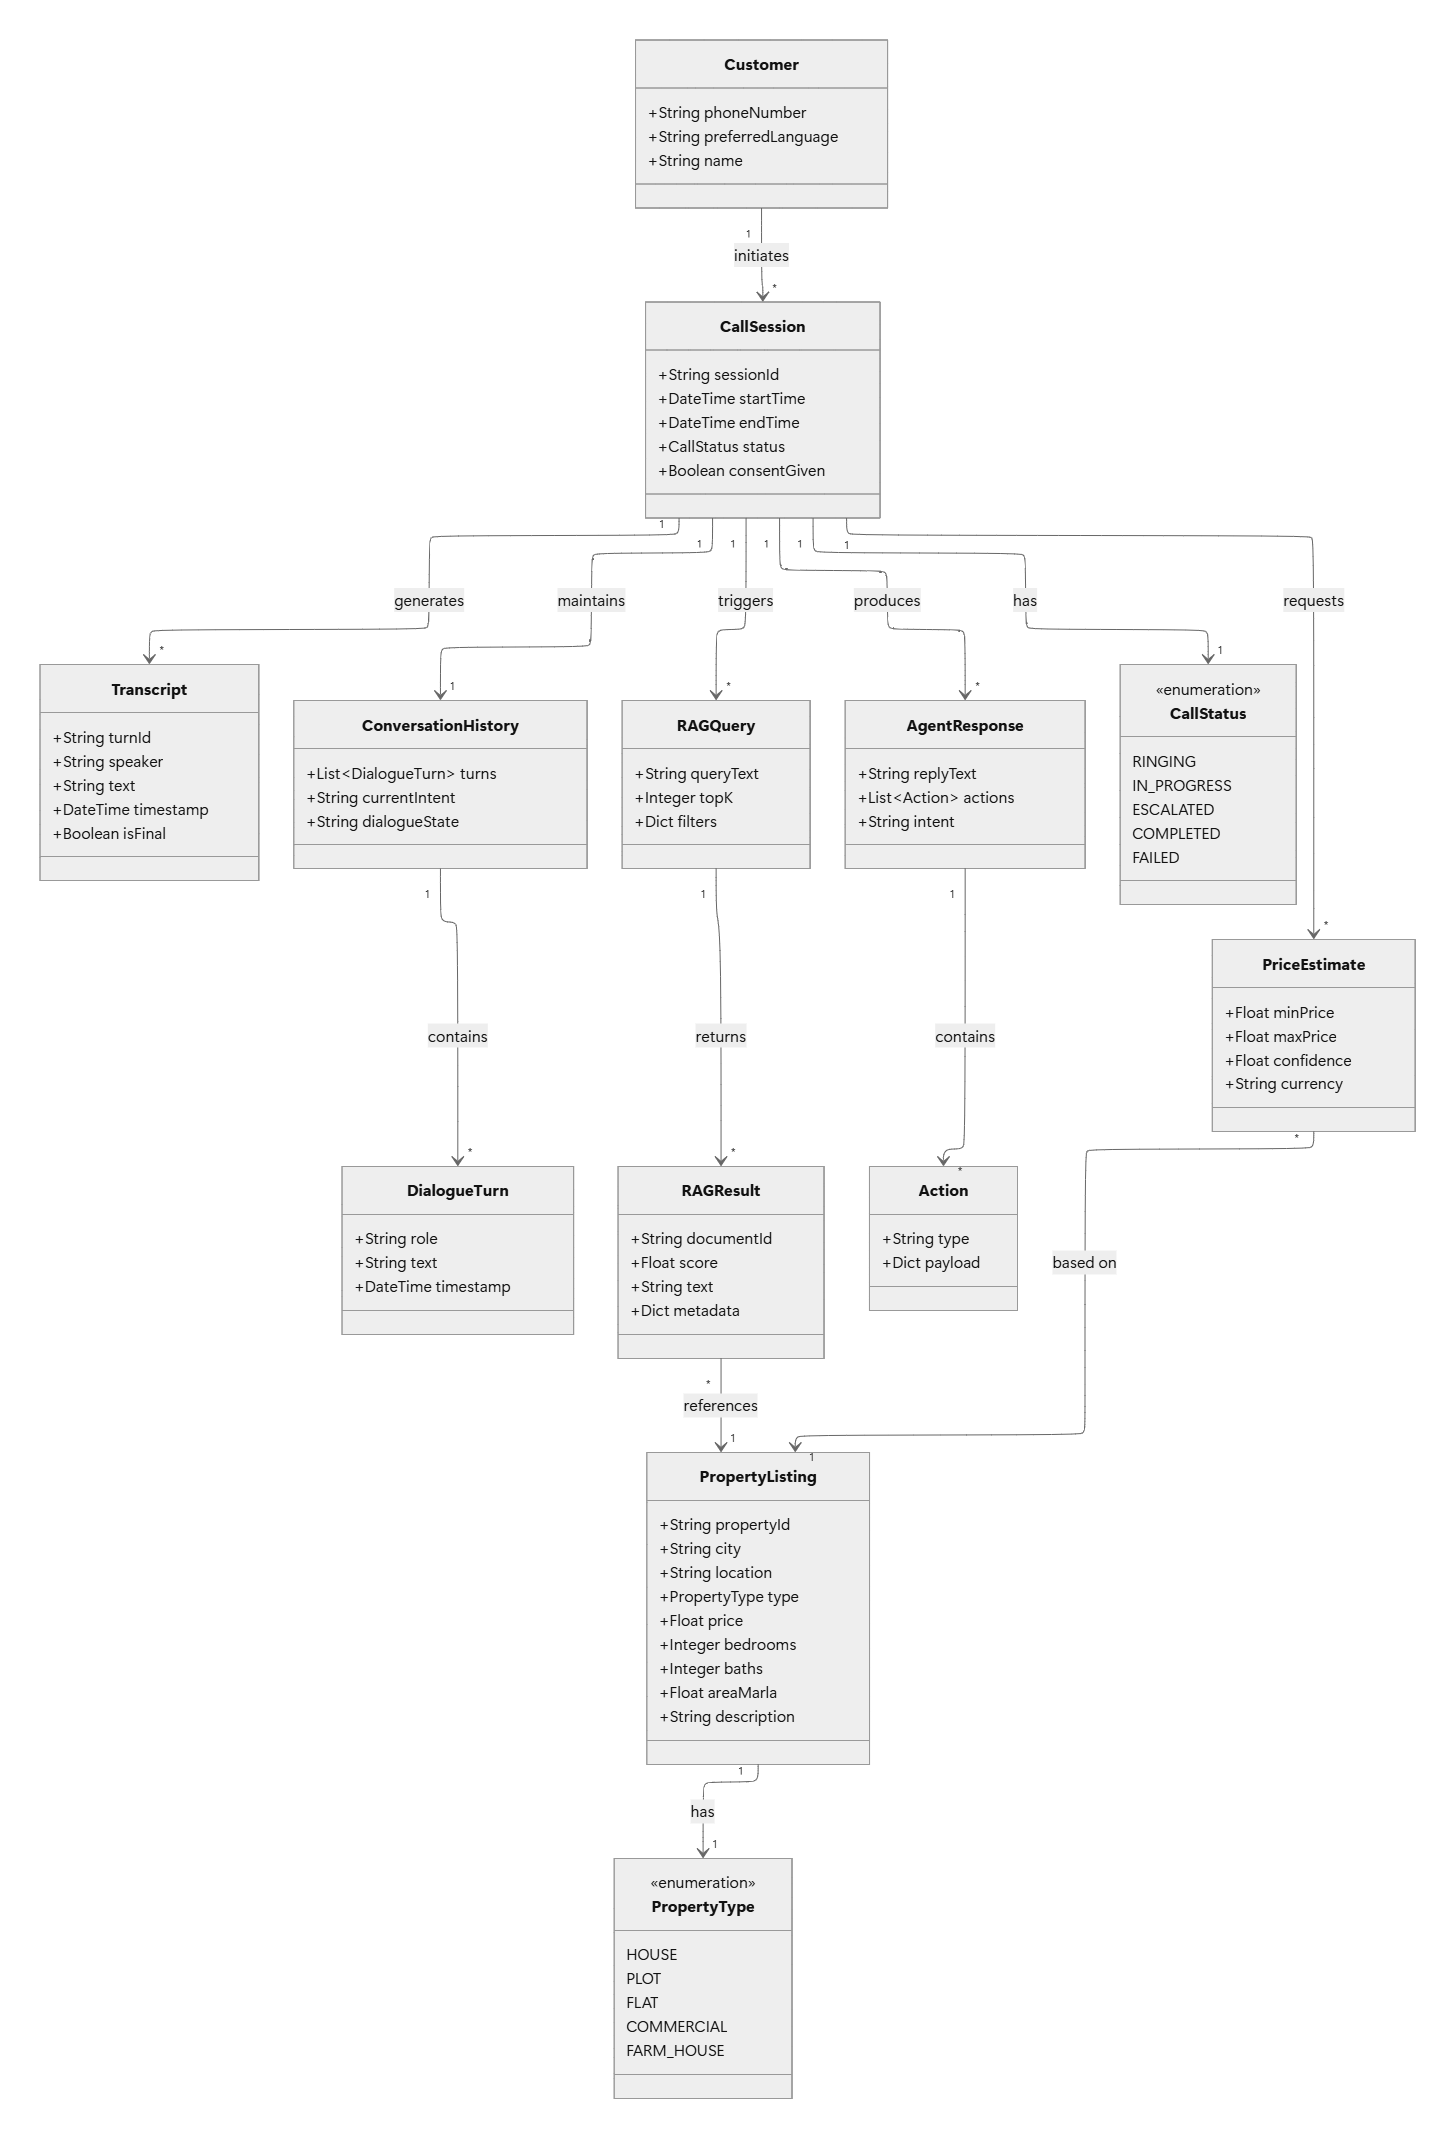
\includegraphics[width=0.95\textwidth]{ThesisFigs/Domain Model Diagram.png}
\caption{Domain Model showing core entities and relationships}
\label{fig:domain-model}
\end{figure}

The model centers on \textbf{CallSession} as the primary entity, linking Customers to Transcripts, RAG queries, and AgentResponses. PropertyListings ground the system's knowledge, while PriceEstimates and Actions enable interactive responses.
